%%%%%%%%%%%%%%%%%%%%%%%%%%%%%%%%%%%%%%%%%%%%%%%%%%%%%%%%%%%%%%%%%%%%%%%%%%
%% Review Volume (last updated on 20-4-2015)                            %%
%% Trim Size: 9in x 6in                                                 %%
%% Text Area: 7.35in (include runningheads) x 4.5in                     %%
%% Main Text: 10 on 13pt                                                %%
%% For support: Yolande Koh, <ykoh@wspc.com.sg>                         %%
%%              D. Rajesh Babu, <rajesh@wspc.com.sg>                    %%
%%%%%%%%%%%%%%%%%%%%%%%%%%%%%%%%%%%%%%%%%%%%%%%%%%%%%%%%%%%%%%%%%%%%%%%%%%
%%
%\documentclass[wsdraft]{ws-rv9x6} % to draw border line around text area
\documentclass{ws-rv9x6}
\usepackage{subfigure}   % required only when side-by-side / subfigures are used
\usepackage{ws-rv-thm}   % comment this line when `amsthm / theorem / ntheorem` package is used
\usepackage{ws-rv-van}   % numbered citation & references (default)
%\usepackage{ws-index}   % to produce multiple indexes
\makeindex
%\newindex{aindx}{adx}{and}{Author Index}       % author index
%\renewindex{default}{idx}{ind}{Subject Index}  % subject index


\newcommand{\TODO}[1]{\textcolor{red}{#1}} % for temporary working notes
\newenvironment{paraphrase}{\color{blue}}{\color{black}} % for text from old paper that needs to be paraphrased



\begin{document}

\chapter[Evaluating Deleted File Recovery (DFR) tools per NIST guidelines]{Evaluating Deleted File Recovery (DFR) tools per NIST guidelines\\ subtitle\label{ra_ch1}}

\author[F. Author and S. Author]{First Author and Second Author\footnote{Author footnote.}}
%\index[aindx]{Author, F.} % or \aindx{Author, F.}
%\index[aindx]{Author, S.} % or \aindx{Author, S.}

\address{CS Department, BGSU,\\
Bowling Green, Ohio, USA 43403, \\
f\_author@bgsu.edu\footnote{Affiliation footnote.}}

\begin{abstract}
The abstract should summarize the context, content and conclusions of
the paper in less than 200 words. It should not contain any references
or displayed equations. Typeset the abstract in 9 pt Times roman with
baselineskip of 11 pt, making an indentation of 1.5 pica on the left
and right margins.
\end{abstract}

%\markboth{Even Page Header}{Odd Page Header} % Customized running heads

\body

%\tableofcontents

\section{Introduction}\label{intro}

\begin{paraphrase}
 Both in corporate and government settings, digital forensic (DF) tools are used for post-mortem investigation of cyber-crimes and cyber-attacks. 
Nowadays it is common~\cite{df:news} for law enforcement to use DF tools to follow an electronic trail of evidence to track down a suspect. 
To maintain the quality and integrity of DF tools, National Institute of Standards and Technology (NIST)'s 
Computer Forensics Tool Testing Program (CFTT)~\cite{cftt:nist} 
defined expectations for these tools. Maintaining the standards of DF tools 
is especially critical for judicial proceedings: usage of a forensic tool that does not follow the standards may cause evidence to be thrown 
out in a court case, whereas incorrect results from a forensic tool can also lead improper prosecution of an innocent defendant. 

The focus of this paper is about standardization of one class of DF 
tools that are for Deleted File Recovery (DFR)~\cite{meta:dfr:standards}. 
As the name suggests, a DFR tool attempts to retrieve deleted files
from a file system of a computer. As an example, given a hard disk or a USB drive 
(which might have been seized from the suspect computer or collected from the crime scene), a 
forensics professional can use a DFR tool to investigate about (and potentially retrieve) files which 
a suspect deleted to hide important information. 
The success or failure of a DFR tool can decide the outcome of a case.  

DFR tools are typically classified as one of two varieties, corresponding to two different approaches to file recovery.
These varieties are \emph{metadata-based} tools and \emph{file carving} tools.
The focus of this paper is metadata-based DFR tools, with file carving left for future work.
In the rest of the paper, unless otherwise mentioned, by \emph{DFR tool} we mean metadata-based DFR tool.

Our experiments with a popular DF tool suite named Autopsy~\cite{autopsy} 
show that it does not meet all NIST expectations for DFR. 
Furthermore, we extensively experimented with other frequently used DFR tools. 
We compare those tools' performance and compile a comparative analysis, which could help the user choose the right DFR tool. 

Evaluating the performance of a DFR tool is complex because many elements of a forensics scenario determine 
the success or failure of the file recovery process. 
A few such factors are the type of the file system (FAT, NTFS, etc.), presence of other active/deleted 
files in the file system, fragmentation of a file, a deleted file being overwritten by another file, and so on.
So, comparison of two DFR tools is scientific only if they are compared while keeping these factors same. 
Via extensive analysis, we design a set of test file system images (for either of FAT and NTFS) which considers each of the above factors independently. 
We claim that this list of test cases cover most of the scenarios (except few edge cases) in real-life, and thus claim that our evaluation has broad coverage. 

As there are many file systems (e.g., ext4, HFS, etc.) in addition to FAT and NTFS, one might be interested to know why we chose FAT and NTFS for the current work. 
Because FAT and NTFS are very widely used on external storage devices and devices running Microsoft Windows, respectively,
real-life forensics investigation often involves these two file systems.
While we leave other file systems for future study, our current methodology could be 
extended to other file systems to make a similar study.

The main contributions of the paper are listed as follows:
\begin{itemize}
\item We design and build a list of canonical test file system (FAT and NTFS) images to evaluate the DFR tool per NIST guidelines. 
\item We perform evaluation of frequently-used DFR tools (including free tools as well as proprietary ones)\footnote{As the subject of our evaluation study, 
we have chosen a few tools or trade names. In no case does such choosing imply recommendation or endorsement by the authors.} on the test images.
\item For the interesting cases of tools' success or failure, we provide logical explanation.
\item We provide critique on applicability of some of the NIST guidelines in a practical setting. 
\end{itemize}


The NIST CFTT portal currently publishes reports of only a subset of DFR tools. 
However, that set needs to be expanded as many new tools come to market and become popular.
Also, existing DFR tools should be retested to ensure their reliability is consistent 
as new patches and features come out. 
Adding new reports to the CFTT website will allow tool developers a 
chance to continually develop their tools for the better. We will submit our study reports to the CFTT portal.
At the time of writing, the portal publishes reports for Autopsy~\cite{dhs:autopsy} and FTK~\cite{dhs:ftk}; 
however, both reports are from 2014 and evaluate now-outdated versions of the software.

As a side benefit, our work leads to a few hands-on lab-modules to be used in digital forensics courses 
at BGSU, enriching the new DF specialization program in the CS department. We will also make these modules
publicly available to be used by relevant instructors at other universities.

\end{paraphrase}




\section{Background}

\begin{paraphrase}
 In this section, we present some of design basics (often simplified to aid readability) of FAT file system and NTFS file system, 
which are relevant to what we discuss in the latter part of the paper. 
We highlight what information remains in the file system after a file is deleted, 
which leads to understanding of how metadata-based file-recovery might work. 
Finally, we present the \emph{core features} of NIST standards for such recovery tools.  
\end{paraphrase}

\TODO{Add a few lines about carving}


\subsection{FAT File System}
\begin{paraphrase}
 As in many other file systems, a file in FAT system has metadata in addition to the actual file content. 
The main metadata of a file (say foo.txt) in FAT system is called a \emph{directory entry}, which is of 32 bytes.
The directory entry of a file (say foo.txt) has three main \emph{essential} elements: (a) file name, (b) file size, and 
(c) index of the starting cluster (which holds the actual file content). We can figure 
out the index of other clusters of the file by reading a global table called the FAT table. The FAT table
can determine the chain of clusters which hold the data of a file. In particular, 
for each cluster (say x) of the file system, the FAT table has an entry, and 
if FAT(x) is 0, then that means cluster x is currently unallocated. 
On the other hand, if FAT(x) is y, then that means cluster y is the next cluster after cluster x (as part of the same file).
If FAT(x) is EOF, that indicates cluster x is the last cluster of the file.
   
As an example, the directory entry of foo.txt and the clusters (holding the actual content of foo.txt) 
are illustrated in Figure~\ref{fig:fat1}. The FAT table is also shown, which tells us that foo.txt's data is stored 
in contiguous clusters, starting from cluster 100 and ending at cluster 200.

% \begin{figure}[h]
%     \centering
%     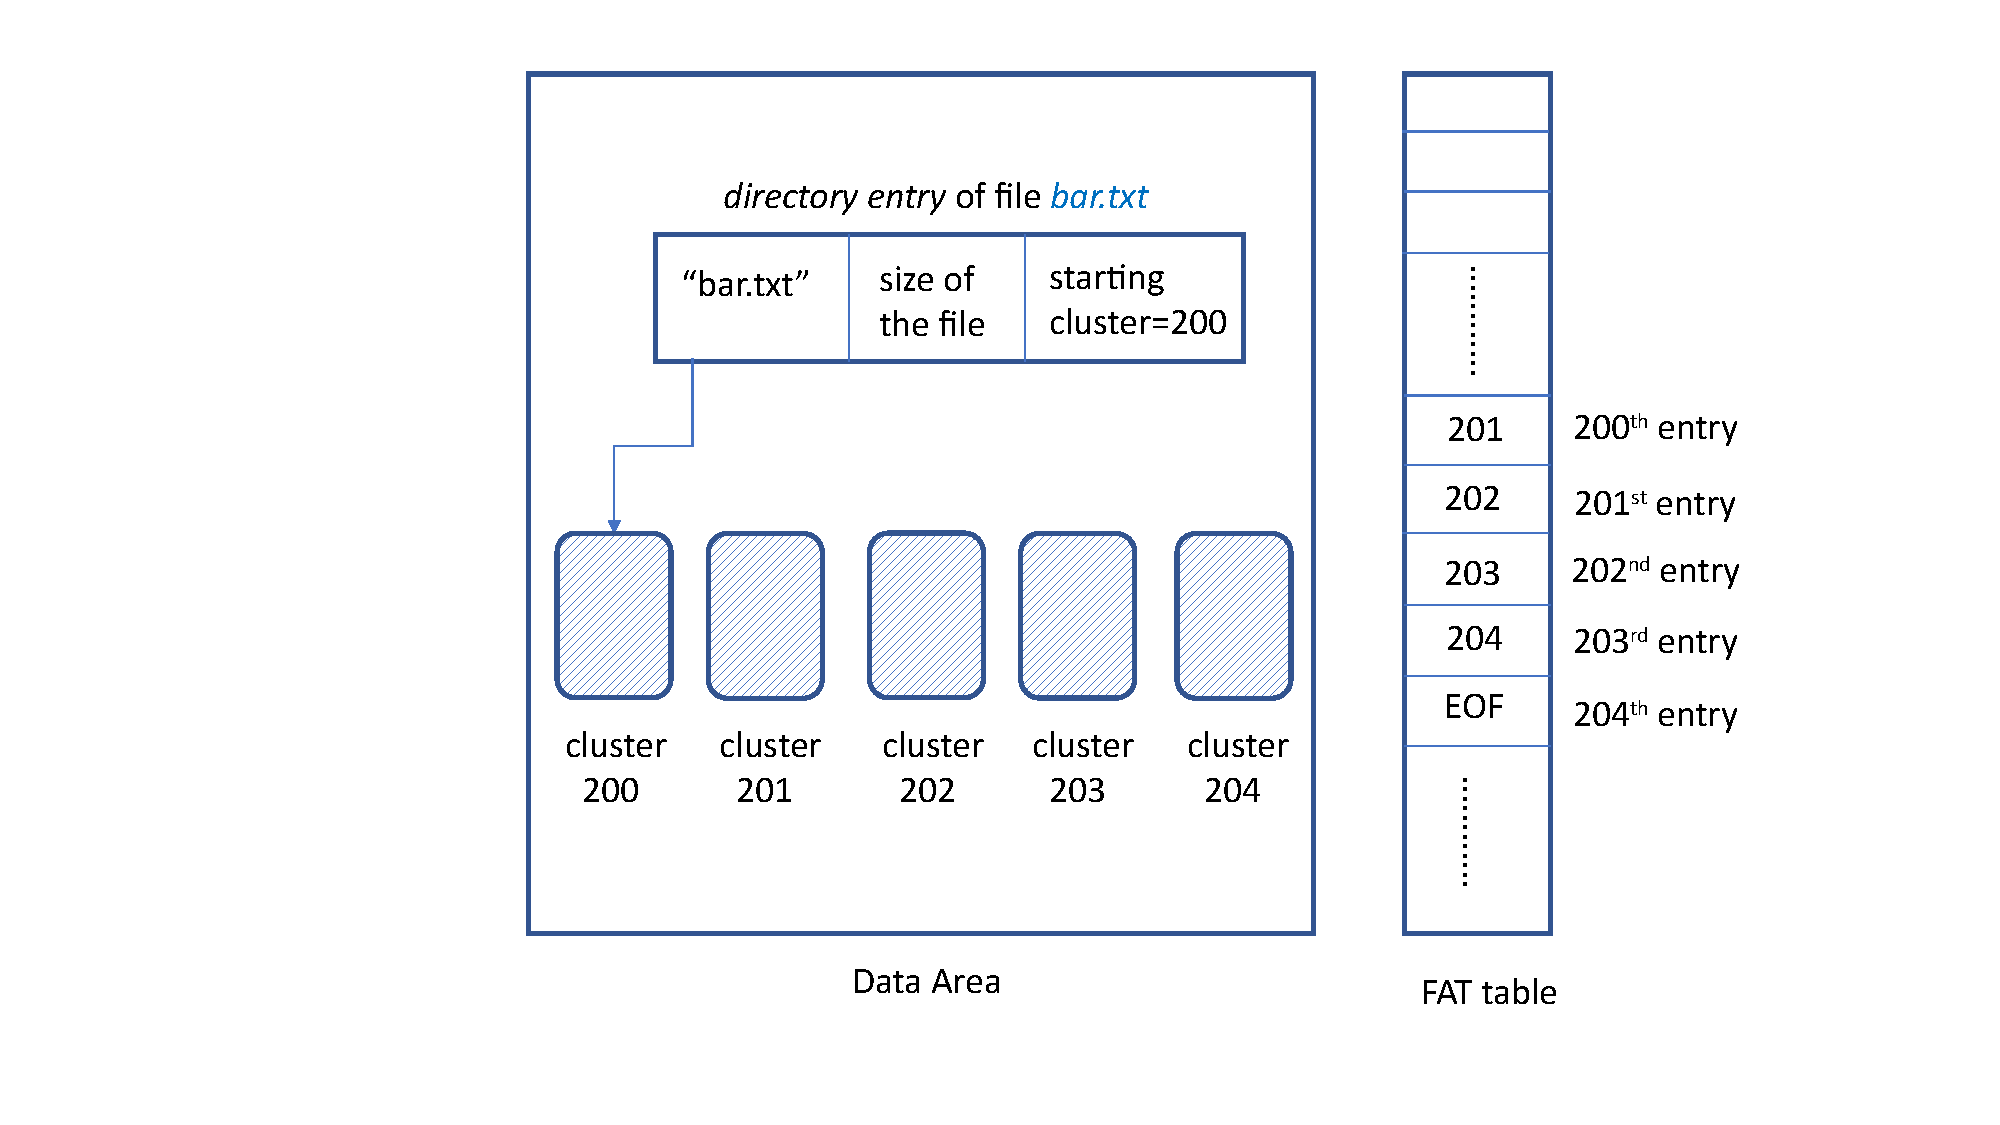
\includegraphics[width=\linewidth]{fig/fat1.pdf}
%     \caption{File foo.txt in a FAT file system. The \emph{directory entry} of this file and the actual file content clusters (shaded) are shown. 
% The FAT table is also shown, which determines the chain of clusters (from cluster 100 to cluster 200) of foo.txt.}
%     \label{fig:fat1}
% \end{figure}


The change in metadata and actual content of foo.txt is illustrated in Figure~\ref{fig:fat2} after the file is deleted.
The first character of the file name (say ``foo.txt") is flagged (``\_oo.txt") to denote that the file is deleted, 
but the remaining part of the directory entry can be still available. In the FAT table, the deleted file's corresponding
entries are \emph{zeroed}, which denotes that those clusters are available to be allocated to a new file (if necessary).
However, the actual content carrying clusters (say cluster 100 to cluster 200)
can still be intact until they are \emph{overwritten} by another file. 
  
% \begin{figure}[h]
%     \centering
%     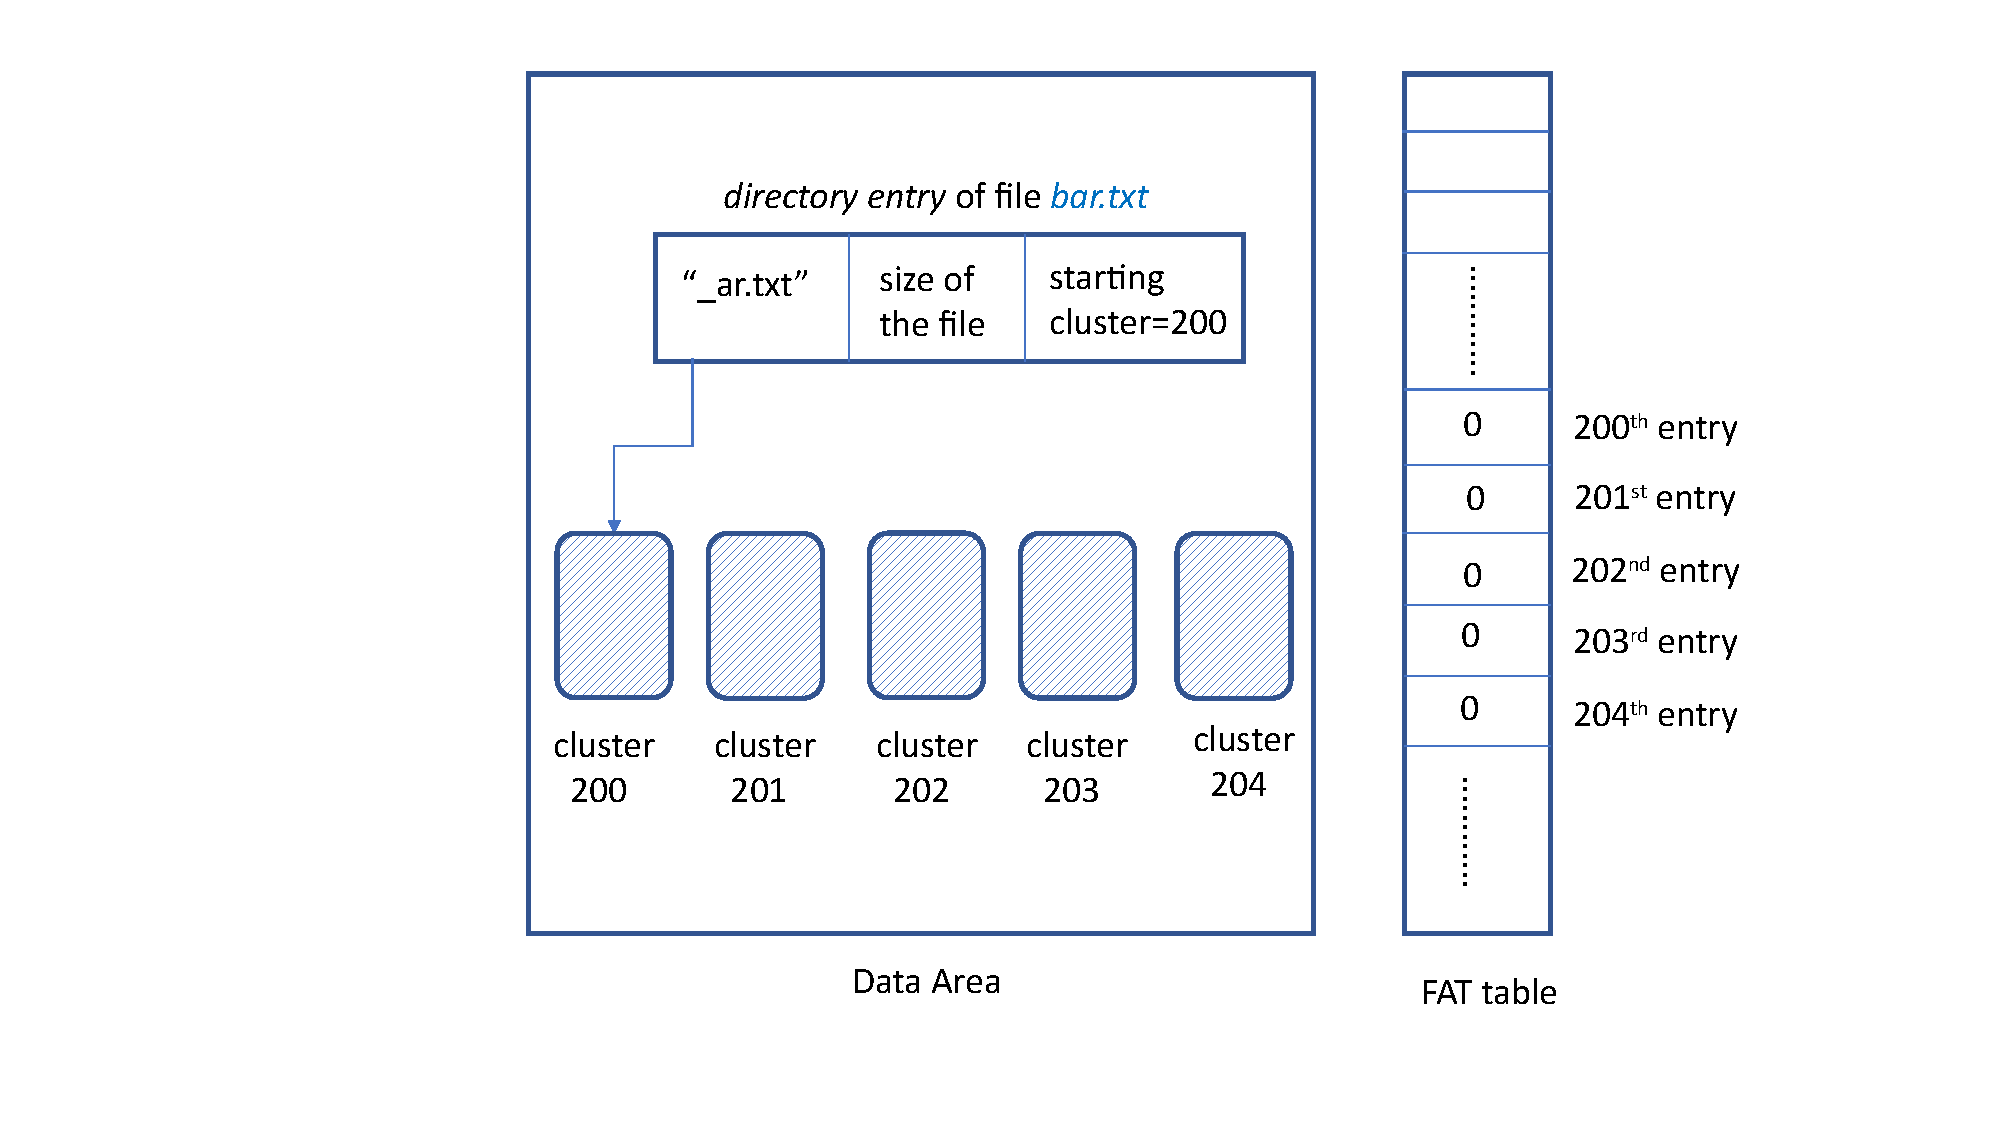
\includegraphics[width=\linewidth]{fig/fat2.pdf}
%     \caption{The metadata and actual content of foo.txt are shown after the file is deleted whereas the corresponding entries (i.e., 100-200) in the FAT table are zeroed.}
%     \label{fig:fat2}
% \end{figure}

Furthermore, it is possible that the content of a file is not stored in contiguous clusters in FAT file system, 
and this phenomenon is called \emph{fragmentation}.
If the original file foo.txt has two fragments, it may look as illustrated in Figure~\ref{fig:fat3} where the file's first fragment is from cluster 100 to cluster 101 and the 
second fragment is from cluster 200 to cluster 298. 

% \begin{figure}[h]
%     \centering
%     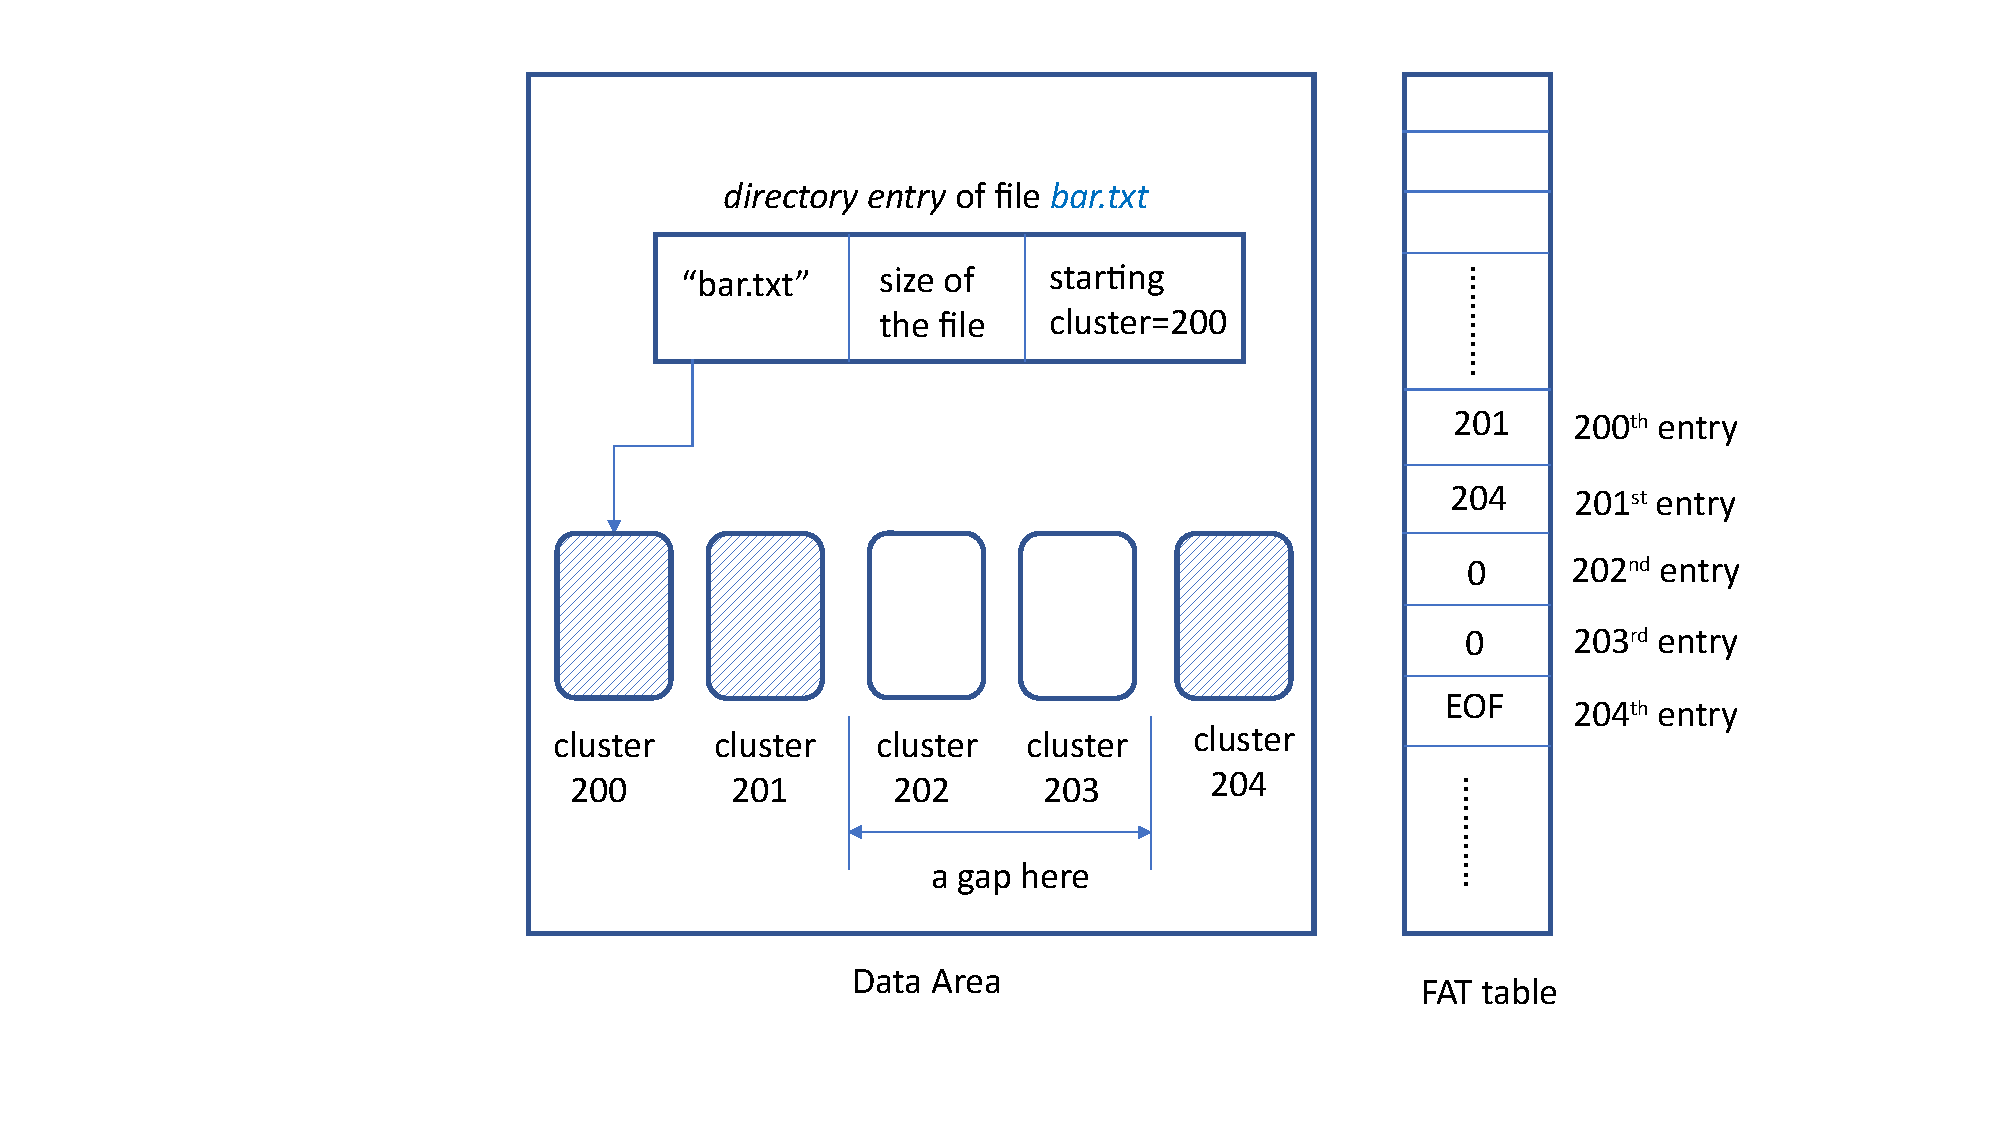
\includegraphics[width=\linewidth]{fig/fat3.pdf}
%     \caption{The layout of metadata and actual content of a file foo.txt is shown whereas the file has two fragments (cluster 100-101 and cluster 200-298) 
% as determined by the FAT table.}
%     \label{fig:fat3}
% \end{figure}
\end{paraphrase}



\subsection{NTFS File System}
\begin{paraphrase}

In an NTFS system, each file has an entry in the Master File Table (MFT) where every entry is typically 1024 bytes. 
If a file is short, then all of its metadata as well as the actual content can sit inside the MFT entry; otherwise, 
the file content can be non-resident (i.e., not in MFT entry) and located in other clusters.
  
As an example, the MFT entry of foo.txt and the actual content carrying clusters are illustrated in Figure~\ref{fig:ntfs}.
The MFT entry indicates that there are two runs of clusters (100-101 and 200-298) which carry the actual file content. 
In this case, the example file has two fragments.

% \begin{figure}[h]
%     \centering
%     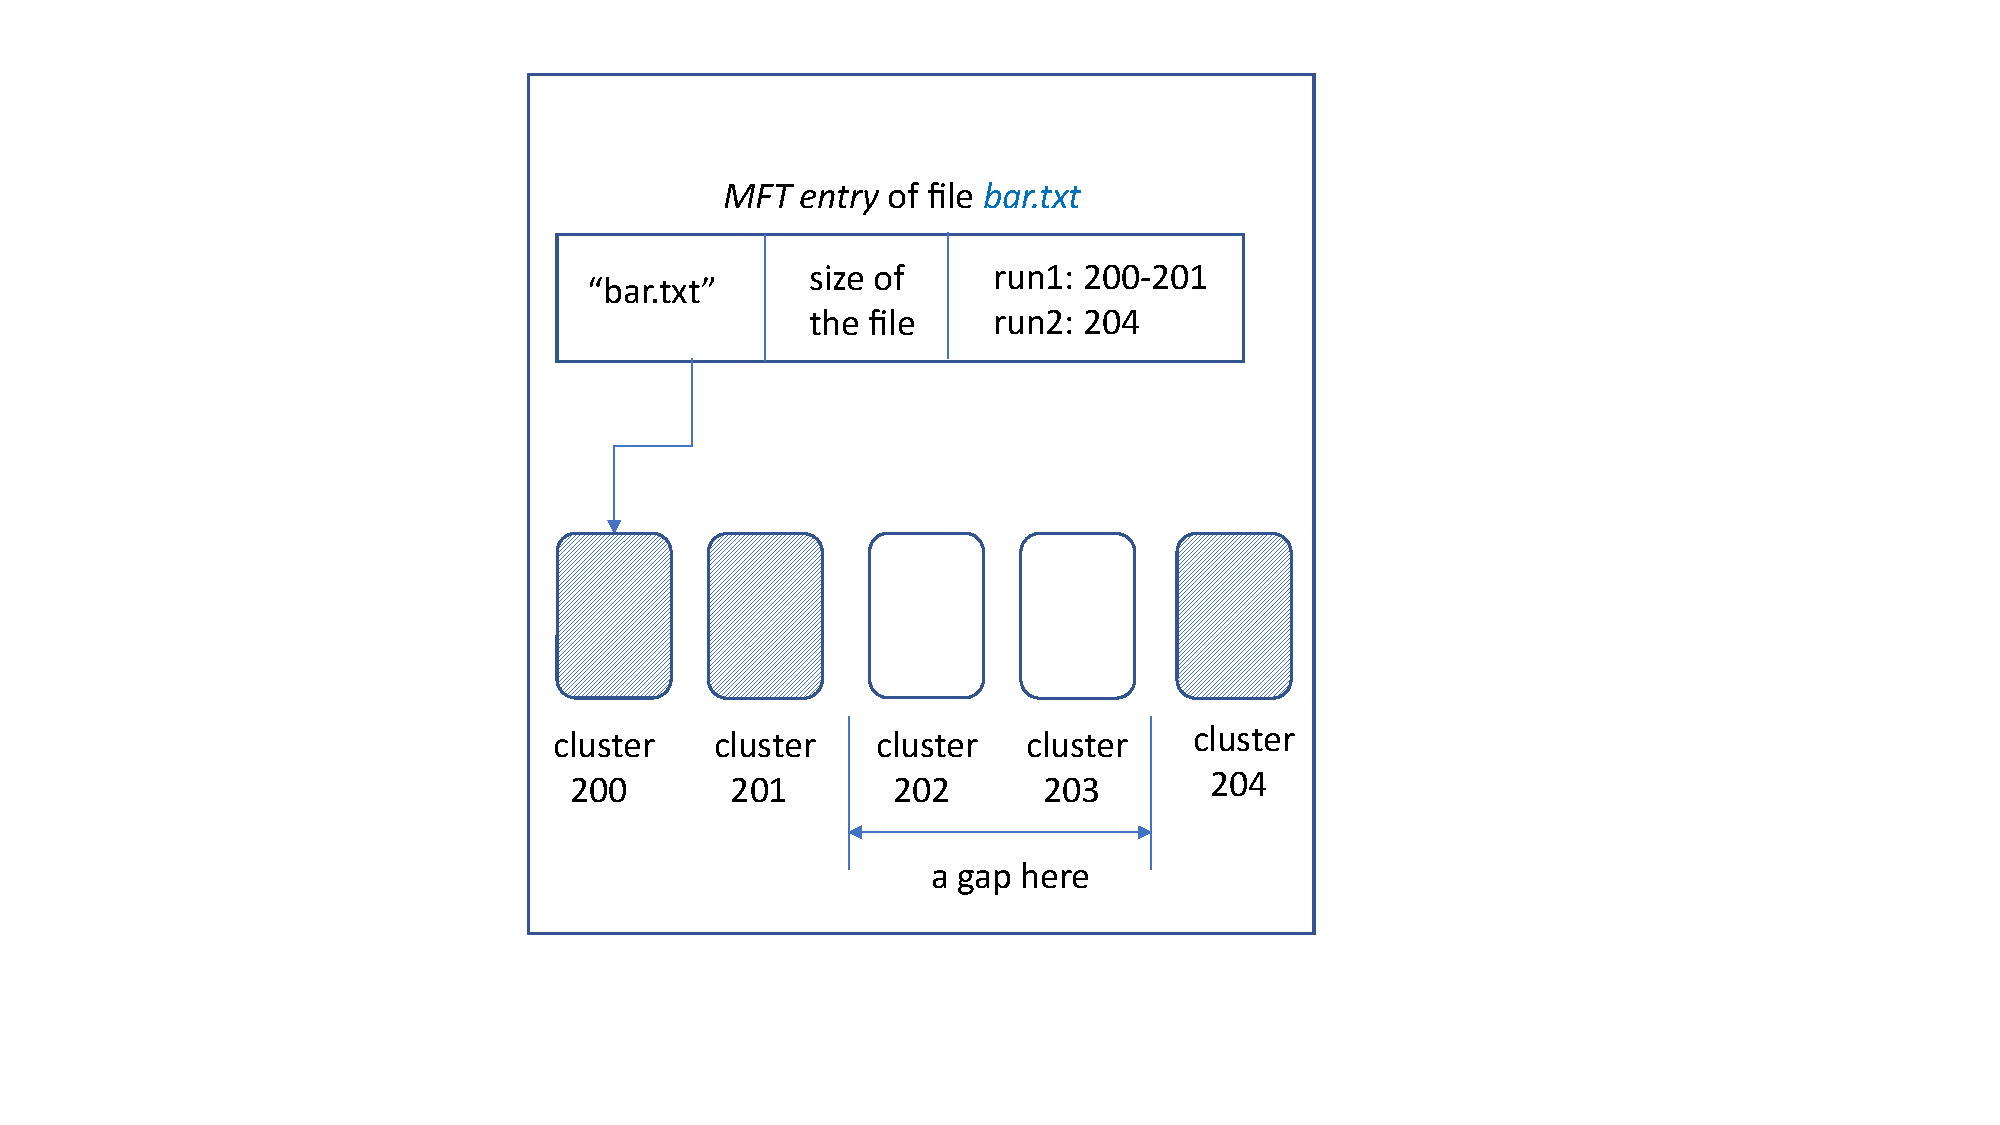
\includegraphics[width=\linewidth]{fig/ntfs.pdf}
%     \caption{To illustrate NTFS file system, the MFT entry of foo.txt and the actual content carrying clusters are shown. 
% This file has two fragments (cluster 100-101 and cluster 200-298).}
%     \label{fig:ntfs}
% \end{figure}
 
\end{paraphrase}

\subsection{Metadata-Based Deleted File Recovery}
\begin{paraphrase}
 The previous discussion implies that in many cases a deleted file's metadata 
(e.g., directory entry in FAT or MFT entry in NTFS) can be still available, 
and it is possible to recover the file content using this metadata. 
This is called metadata-based deleted file recovery.

For instance, in the example of Figure~\ref{fig:fat2},
we can see from the directory entry of foo.txt that 
the deleted file starts in cluster 100 and has a size of 101 clusters;
thus, we can reason that the deleted file content is in cluster 100 to cluster 200.
We can recover the whole file via reading the raw content of these clusters (e.g., by using dd command in Kali Linux). 

Note that in FAT system the \emph{directory entry} of a file only refers to the starting cluster, and it does not carry any information about the file fragments.
That is why in certain situations where the deleted file is fragmented, metadata-based file recovery in FAT system encounters challenges.
On the other hand, if a file is fragmented in NTFS, the corresponding MFT entry does contain information on all the runs (i.e., fragments) of the file
(as shown in Figure~\ref{fig:ntfs}). Consequently, fragmentation does not introduce any extra challenge in file recovery in NTFS.
\end{paraphrase}

\subsection{File Carving}

\TODO{TODO}

\subsection{NIST Guidelines}
\subsubsection{For Metadata-Based DFR}
\begin{paraphrase}
 The NIST guidelines~\cite{meta:dfr:standards} list four \emph{core features} upon which metadata-based DFR tools are to be judged.
Following is the text of each core feature as well as our interpretation of each in the context of this work:
\begin{enumerate}
 \item ``The tool shall identify all deleted File System-Object entries accessible in residual metadata''~\cite{meta:dfr:standards}.
 We consider a tool passing this standard if it identifies to the user each file system metadata entry that is marked as deleted.
 \item ``The tool shall construct a Recovered Object for each deleted File System-Object entry accessible in residual metadata''~\cite{meta:dfr:standards}.
 We consider a tool passing this standard as long as it outputs a file for each deleted file, even if the output file is empty.
 \item ``Each Recovered Object shall include all non-allocated data blocks identified in a residual metadata entry''~\cite{meta:dfr:standards}.
 For FAT file systems, we consider a tool passing this standard if it recovers at least the first contiguous segment of unallocated sectors starting 
from the first sector originally allocated to the deleted file. For NTFS file systems, the tool must recover all unallocated sectors originally allocated to the deleted file.
 \item ``Each Recovered Object shall consist only of data blocks from the Deleted Block Pool''~\cite{meta:dfr:standards}.
 We consider a tool passing this standard if the recovered file consists only of data from the original deleted file, or null data to represent omitted portions.
\end{enumerate}
\end{paraphrase}

\subsubsection{For File Carving}

\TODO{TODO}

\section{Research Questions}

\begin{paraphrase}
A DFR tool is a piece of software that can retrieve residual data of a file that was deleted 
from a storage device (e.g., computer hard disk, flash drive, and so on). We evaluate a set of 
popular DFR tools on the scale of CFTT guidelines. 
In particular, following are the research questions (RQs) that we target to answer. 

\begin{itemize}
\item[RQ1.] Do the popular metadata-based DFR tools meet the NIST CFTT expectation? 
If not, which tool meets which part of the expectation? 

\item[RQ2.] What factors make the metadata-based tools fail or succeed?

\item[RQ3.] Do the popular file carving tools meet the NIST CFTT expectation? 
If not, which tool meets which part of the expectation? 

\item[RQ4.] What factors make the file carving tools fail or succeed?

% \item[RQ5.] Are the free DFR tools more effective compared to the enterprise-level (proprietary) tools? \TODO{still include this?}
\end{itemize}

The identification of errors, such as for not recovering a deleted file or attempting to recover a file that was never there 
(Type I and Type II errors, respectively), is an important metric for a DFR tool. 
Type I and Type II errors account for majority of the standard. Many factors impact the performance of a DFR tool, 
including file system type, whether the file content is not located in contiguous clusters, whether 
some part of the deleted file content is overwritten by another file, and more.
We consider these variables in the design of experiment when we compare the tools.
Note that our current study is limited to exploring the \emph{core features} of NIST guidelines~\cite{meta:dfr:standards}, 
i.e., we leave the optional features~\cite{meta:dfr:standards} of NIST guidelines for future study. \TODO{work carving into this paragraph}
\end{paraphrase}




\section{Approach}
\subsection{Overview}
\begin{paraphrase}
 To test the DFR tools, we first design hypothetical test scenarios to simulate the challenges of real-world file recovery.
We then create each scenario in real file systems and save them as raw images. 
Using the images as input, we run each DFR tool and attempt to recover all deleted files. 
Finally, we compare the recovered files to their original versions in order to judge the tools' 
meeting with the NIST expectation. A high-level view of the methodology for a typical test case is illustrated in Figure~\ref{fig:overview}.

% \begin{figure}[h]
%     \centering
%     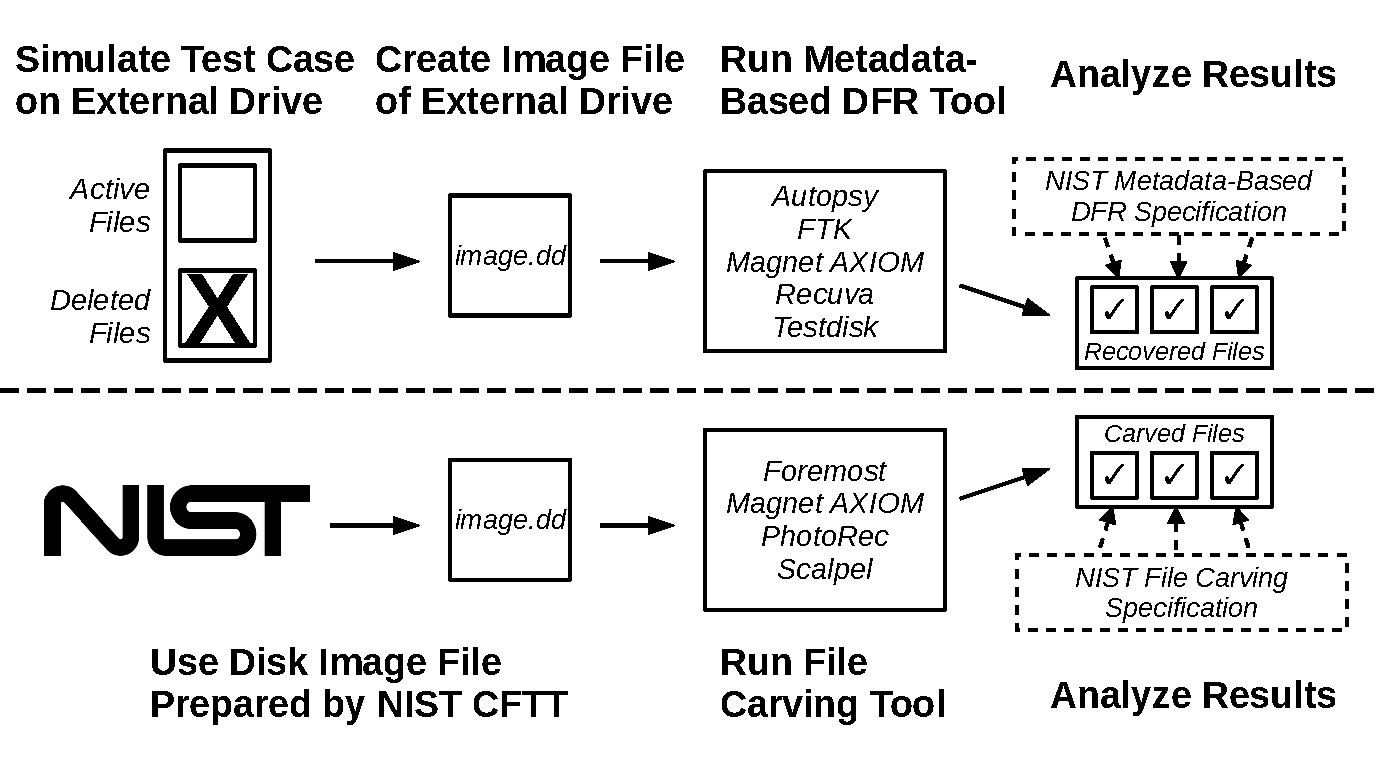
\includegraphics[width=\linewidth]{fig/overview.pdf}
%     \caption{A file system containing deleted files is created on the external drive. 
% The drive's raw data is then saved as a read-only file, called a \emph{disk image} or \emph{file system image}.
% The disk image is given as input to a DFR tool, which attempts to recover the deleted files. 
% The recovered files are then analyzed to judge the DFR tool's meeting with the NIST CFTT expectation.}
%     \label{fig:overview}
% \end{figure}
\end{paraphrase}


\subsection{Metadata-Based Tools}
\subsubsection{Designing Recovery Scenarios}
\begin{paraphrase}
 To test the DFR tools' meeting with the expectation, we designed a variety of scenarios in which a tool might have to recover a deleted file. 
We started with the simplest possible case: a file system containing just one deleted file. 
This case is ideal and trivial, but by adding more files, we can create a greater variety of scenarios.

The NIST guidelines limit their scope to recovery of files which were ``created and deleted in a process similar to 
how an end-user would create and delete files,''~\cite{meta:dfr:standards} and exclude 
``files and file system metadata that is specifically corrupted, modified, or otherwise manipulated to appear deleted.''~\cite{meta:dfr:standards}
In other words, these guidelines address situations in which files were deleted via normal file system operations as 
implemented by a typical operating system, as opposed to direct modification of the file system by a user.
Within these constraints, there are two factors which can significantly complicate the file recovery process: 
fragmentation, and overwriting. 

These factors are thus the foundation of our test scenarios, with all cases besides the first involving either fragmented files, overwritten files, or a combination of both. 
The goal is to create test cases which are canonical; in other words, they constitute the basic elements of a file recovery scenario.
We suggest such a canonical list of test cases should be considered representative of wide variety of scenarios within the scope of the guidelines.

Following are descriptions of the test cases we designed. 
We have separated them into five categories: 
{\bf(a)} a case with just a simple deleted file, 
{\bf (b)} cases involving fragmentation,
{\bf (c)} cases involving overwritten files,
{\bf (d)} cases with a combination of fragmentation and overwriting,
and {\bf (e)} cases with a file fragmented ``out of order.''

When test cases are illustrated in figures, each row represents the file system at a point in time. An arrow indicates a change in the file system, which is illustrated in the following row. Files are distinguished by unique letters, and if they are deleted they are marked as such.

\paragraph{Simple Deleted File}
\begin{itemize}%[align=parleft, labelwidth=4em, leftmargin =\dimexpr\labelwidth+\labelsep\relax]
    \item [Case 1] The file system contains a single deleted file.
\end{itemize}
\paragraph{Deleted File is Fragmented}
\begin{itemize}%[align=parleft, labelwidth=4em, leftmargin =\dimexpr\labelwidth+\labelsep\relax]
%     \begin{figure}[h]
%         \centering
%         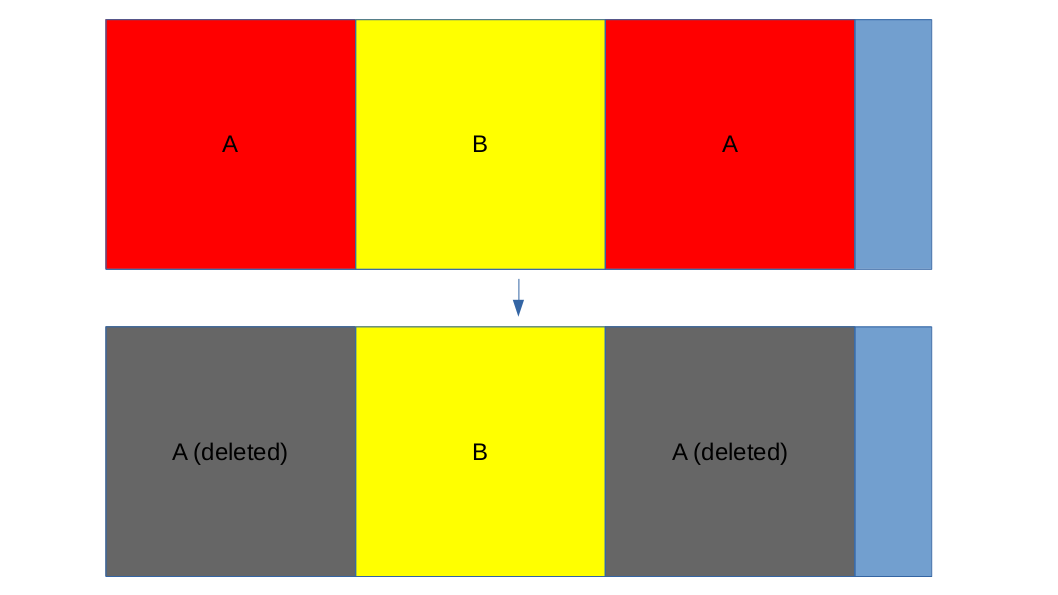
\includegraphics[width=\linewidth]{fig/case2.png}
%         \caption{Test Case 2. Fragmented file A is deleted.}
%         \label{fig:case_2}
%     \end{figure}
    \item [Case 2] Fragmented deleted file, with an active file in between the fragments (as illustrated in Figure~\ref{fig:case_2})
    \item [Case 3] Fragmented deleted file, with a deleted file in between the fragments
\end{itemize}
\paragraph{Deleted File is Overwritten}
\begin{itemize}%[align=parleft, labelwidth=4em, leftmargin =\dimexpr\labelwidth+\labelsep\relax]
%     \begin{figure}[h]
%         \centering
%         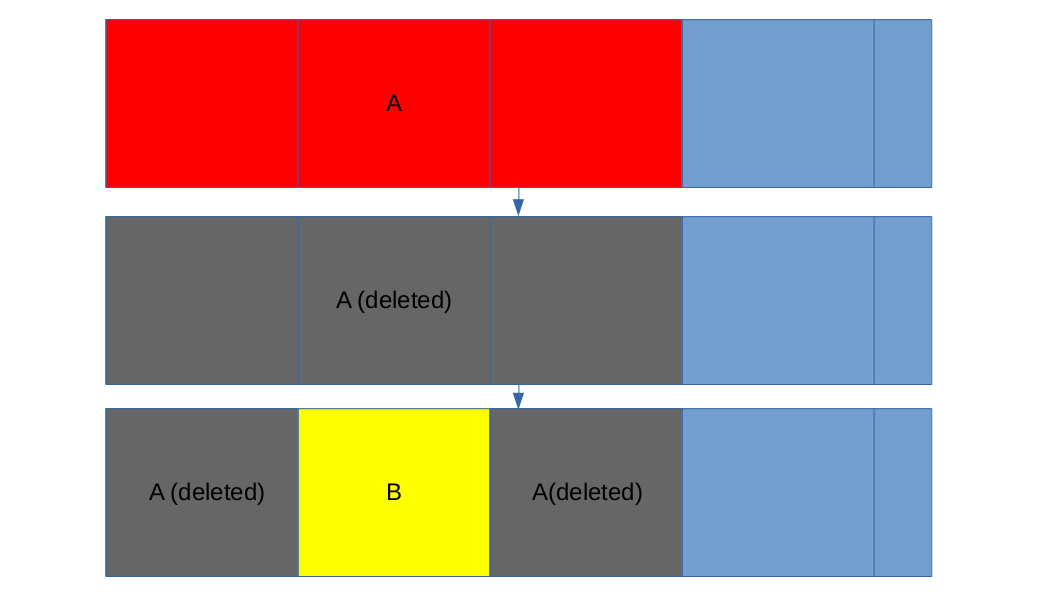
\includegraphics[width=\linewidth]{fig/case4ii.png}
%         \caption{Test Case 4ii. Deleted file A is partially overwritten by active file B.}
%         \label{fig:case_4ii}
%     \end{figure}
    \item [Case 4i] Beginning of deleted file overwritten by an active file
    \item [Case 4ii] Middle of deleted file overwritten by an active file (as illustrated in Figure~\ref{fig:case_4ii})
    \item [Case 4iii] Deleted file partially overwritten by an active file which doesn't end on a sector boundary
    \item [Case 4iv] Deleted file entirely overwritten by an active file
    \item [Case 5i] Beginning of deleted file overwritten by another deleted file (as illustrated in Figure~\ref{fig:case_5i})
    \item [Case 5ii] Middle of deleted file overwritten by another deleted file
    \item [Case 5iii] Deleted file partially overwritten by a deleted file which doesn't end on a sector boundary
    \item [Case 5iv] Deleted file entirely overwritten by a deleted file
\end{itemize}
\paragraph{Deleted File is Fragmented and Overwritten}
 \begin{itemize}%[align=parleft, labelwidth=4em, leftmargin =\dimexpr\labelwidth+\labelsep\relax]
%      \begin{figure}[h]
%         \centering
%         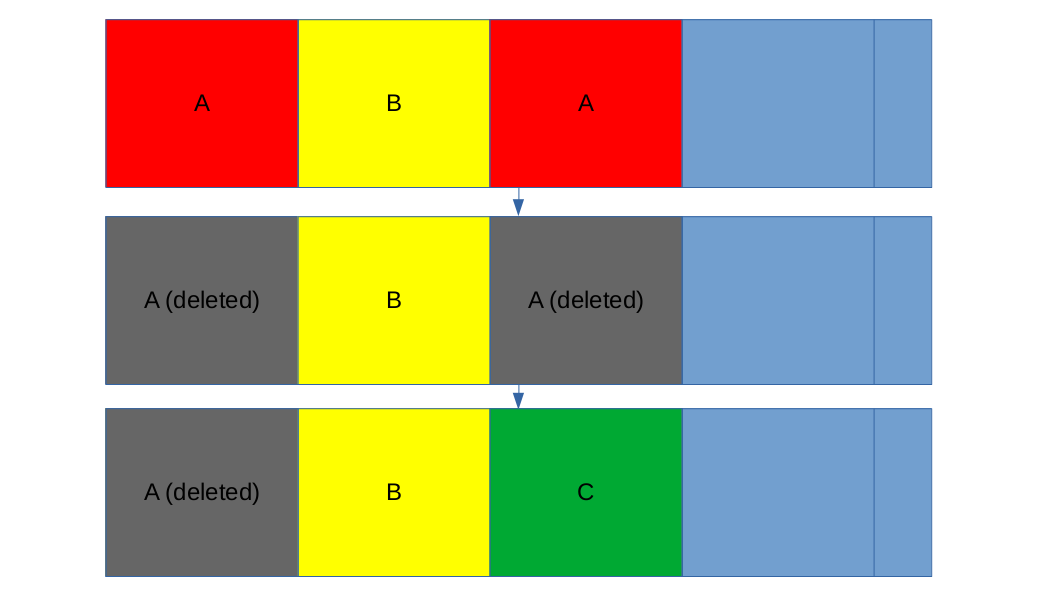
\includegraphics[width=\linewidth]{fig/case6.png}
%         \caption{Test Case 6. Fragmented file A is deleted. File A is then partially overwritten by file C.}
%         \label{fig:case_6}
%     \end{figure}
    \item [Case 6] Fragmented deleted file, with an active file in between the fragments, with the second fragment overwritten by another active file (as illustrated in Figure~\ref{fig:case_6})
    \item [Case 7] Fragmented deleted file, with an active file in between the fragments, with the second fragment overwritten by another deleted file
 \end{itemize}
\paragraph{Deleted File is Fragmented Out-of-Order}
\begin{itemize}%[align=parleft, labelwidth=4em, leftmargin =\dimexpr\labelwidth+\labelsep\relax]
%     \begin{figure}[h]
%         \centering
%         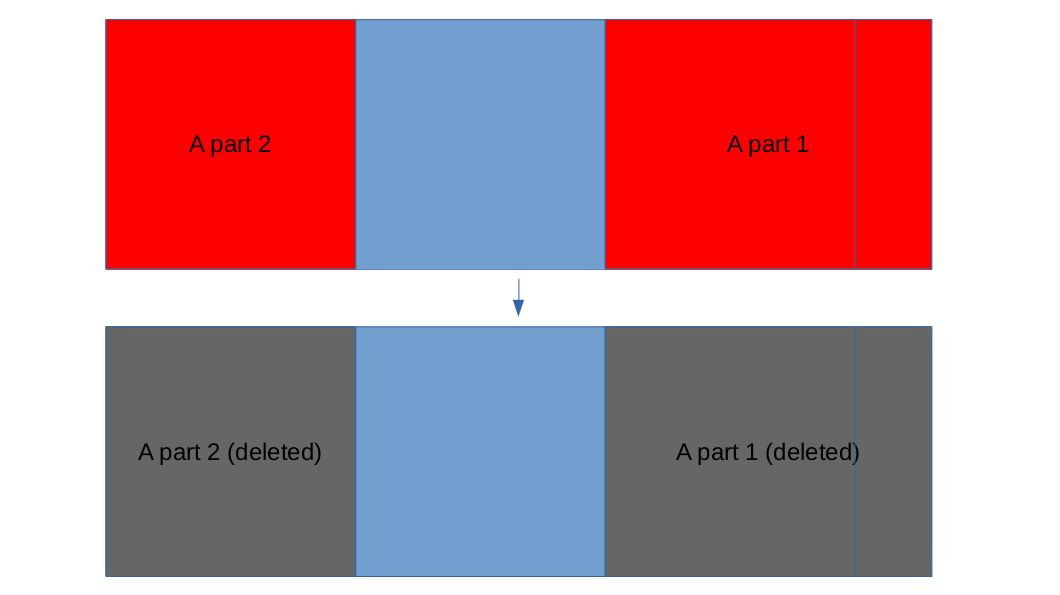
\includegraphics[width=\linewidth]{fig/case8.png}
%         \caption{Test Case 8. Fragmented file A, which starts at the end of the file system and wraps around to the beginning, is deleted.}
%         \label{fig:case_8}
%     \end{figure}
    \item [Case 8] Deleted file fragmented from the end of the file system to the beginning (as illustrated in Figure~\ref{fig:case_8})
    \item [Case 9] Deleted file fragmented from the end of the file system to after an active file
    \item [Case 10] Deleted file fragmented from the end of the file system to after a deleted file
\end{itemize}

Because NTFS keeps track of the locations of all parts of a file even after deletion, fragmentation is not particularly interesting. Cases 8, 9, and 10 would be redundant with case 2, so we have excluded them for NTFS. Due to how NTFS allocates space for files, cases 4ii and 5ii cannot occur as a result of normal file operations, so they have also been excluded. No cases are excluded for FAT tests.
\end{paraphrase}


\subsubsection{Creating Test Images}

\begin{paraphrase}
 All test file systems were created in partitions on a 32 GB flash drive. For each test case, the first step is to entirely write over the partition with zeros. This ensures all cases start from identical, reproduceable conditions. A new file system is written to the partition, then files are written to the file system and deleted. The files used are simple text files containing one letter repeated (e.g., ``aa1M'' is 1 MiB of the letter `a'). Files are written to the test file system by simply copying them from another drive. In some cases we also append data to a file in the test file system to create fragmentation. Once the test file system matches the intended scenario, a read-only image of the partition is created. All tests are performed on these images rather than the original drive. Note that when creating FAT test cases we use Ubuntu 18.04 and for NTFS test cases we use Windows 10.
\end{paraphrase}


\subsubsection{Challenges}

\begin{paraphrase}
 % Caching problem
It is important to consider when creating test images that the low-level behavior of file operations is not always obvious. For example, when writing a file, there is no guarantee the file's data will be immediately written to the disk. The operating system may cache the operation and wait until the optimal time to perform the write, in order to maximize system performance. We observed this early on, as writing a file and subsequently deleting it would always result in the file's metadata being written, but often left no evidence of the file's data having ever existed. This behavior is obviously undesirable because it leaves nothing meaningful to be recovered. We resolved this by using the \emph{sync} system call, which causes any such cached data to be immediately written to the disk, in between file writes and deletions. Unmounting the file system after writes has a similar effect.

% Learning and using the allocation algorithms
Another type of low-level behavior relevant to the image creation process is the allocation algorithm. The operating system must have some kind of algorithm to decide where in the data area new files should be written. Common allocation algorithms include ``first available,'' ``next available,'' and ``best fit.''
Learning and understanding whatever algorithm the OS uses is very helpful for forcing a specific arrangement of files. We observed that when writing to a FAT file system, Linux uses a ``next available'' algorithm. After the file system is mounted, the first write will start at the first free space in the data area. The next file will be written starting from the first free space after the previous file.
Meanwhile, when writing to an NTFS file system, Windows 10 appears to use a ``best fit'' algorithm. In this case, Windows tries to find the smallest space in which the file can fit without being fragmented, and write it there.
\end{paraphrase}

\subsubsection{Recovering Files}
\begin{paraphrase}
 We selected five popular DFR tools for testing: Autopsy~\cite{autopsy}, Recuva~\cite{recuva}, FTK Imager~\cite{ftk}, TestDisk~\cite{testdisk}, and Magnet AXIOM~\cite{axiom}. 
Note that Autopsy uses a set of DF tools known as The Sleuth Kit (TSK) for metadata-based recovery, so TSK is also implicitly covered by this study. 
These tools were chosen based on popularity and availability.
We also made sure to choose a combination of free and proprietary tools, in order to address one of the research questions.

% \begin{figure*}[h]
%     \centering
% 
%     \begin{subfigure}{0.17\linewidth}
%         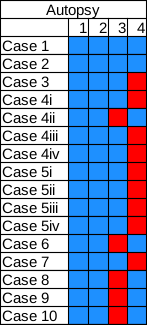
\includegraphics[width=\linewidth]{fig/autopsy_results_fat.png}
%         \subcaption{Autopsy}
%     \end{subfigure}~~
%     \begin{subfigure}{0.17\linewidth}
%         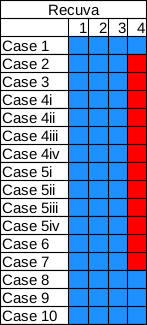
\includegraphics[width=\linewidth]{fig/recuva_results_fat.png}
%         \subcaption{Recuva}
%     \end{subfigure}~~
%     \begin{subfigure}{0.17\linewidth}
%         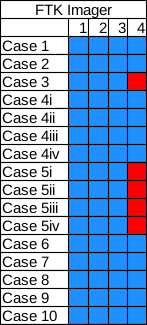
\includegraphics[width=\linewidth]{fig/ftk_results_fat.png}
%         \subcaption{FTK}
%     \end{subfigure}~~
%     \begin{subfigure}{0.17\linewidth}
%         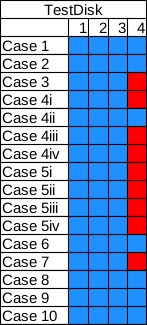
\includegraphics[width=\linewidth]{fig/testdisk_results_fat.png}
%         \subcaption{TestDisk}
%     \end{subfigure}~~
%     \begin{subfigure}{0.17\linewidth}
%         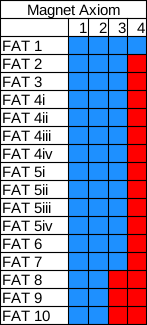
\includegraphics[width=\linewidth]{fig/axiom_results_fat.png}
%         \subcaption{Magnet AXIOM}
%     \end{subfigure}~~
%         
%     \caption{Test results on FAT test cases for each DFR tool. Rows represent test cases whereas columns represent NIST core features. Blue is passing, red is failing, gray is not tested.}
%     \label{fig:results_fat}
% \end{figure*}
% 
% \begin{figure*}[h]
%     \centering
% 
%     \begin{subfigure}{0.17\linewidth}
%         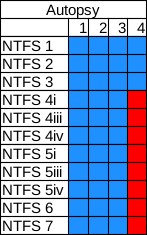
\includegraphics[width=\linewidth]{fig/autopsy_results_ntfs.png}
%         \subcaption{Autopsy}
%     \end{subfigure}~~
%     \begin{subfigure}{0.17\linewidth}
%         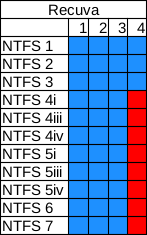
\includegraphics[width=\linewidth]{fig/recuva_results_ntfs.png}
%         \subcaption{Recuva}
%     \end{subfigure}~~
%     \begin{subfigure}{0.17\linewidth}
%         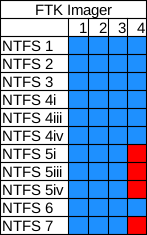
\includegraphics[width=\linewidth]{fig/ftk_results_ntfs.png}
%         \subcaption{FTK}
%     \end{subfigure}~~
%     \begin{subfigure}{0.17\linewidth}
%         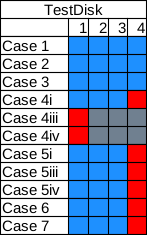
\includegraphics[width=\linewidth]{fig/testdisk_results_ntfs.png}
%         \subcaption{TestDisk}
%     \end{subfigure}~~
%     \begin{subfigure}{0.17\linewidth}
%         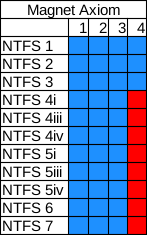
\includegraphics[width=\linewidth]{fig/axiom_results_ntfs.png}
%         \subcaption{Magnet AXIOM}
%     \end{subfigure}~~
%         
%     \caption{Test results on NTFS test cases for each DFR tool. Rows represent test cases whereas columns represent NIST core features. Blue is passing, red is failing, gray is not tested.}
%     \label{fig:results_ntfs}
% \end{figure*}

The settings we used when testing each tool are as follows:
For Autopsy, we performed a standard recovery with all ingest modules disabled.
For Recuva we performed a standard recovery using the free version with default settings.
For FTK Imager, we performed a standard recovery using the free version with default settings.
For TestDisk we used the ``file undelete'' feature under ``Advanced Filesystem Utils.''
For Magnet AXIOM we performed a ``full scan'' in AXIOM Process and exported all files accessible in ``Filesystem View'' in AXIOM Examine.
\end{paraphrase}

\subsubsection{Results}
\begin{paraphrase}
 After testing each tool, we analyzed the recovered object(s) from each test case. 
If the recovered file is identical to the original, obviously all expectations have been met. 
While this is ideal, it is often impossible to perfectly recover a file (such as when it is overwritten) so the standards do not require it. 

In our results, the file is only ever recovered perfectly in FAT cases 1 and 2, and NTFS cases 1-3. 
For all other cases, the tool is judged on each core feature individually. 
These judgments are summarized in Figure~\ref{fig:results_fat} for FAT test cases and Figure~\ref{fig:results_ntfs} for NTFS test cases.

For cases in which a tool does not fulfill core feature 1, in other words, it cannot find a deleted file, we make no judgment about the remaining core features.

\paragraph{Recovering Fragmented Files}
In cases of fragmentation in FAT file systems, we found each tool generally approaches recovery in one of two ways. 
Recuva and Magnet AXIOM start from the beginning of the file and recover the full length of the file even if an active file exists in that space. 
Autopsy, FTK, and TestDisk will start from the beginning of the file and recover the full length, but skip over any active files they encounter.
Autopsy, FTK, and TestDisk recover all of file A, while Recuva and Magnet AXIOM's recovered images erroneously contain data from file B, causing them to fail core feature 4. 
When the space in between fragments is unallocated, all tools recover the file as though it was contiguous, pulling some erroneous data and failing core feature 4. 
When the fragmentation occurs at the end of the file system, Recuva, FTK, and TestDisk recover only the first fragment, while Autopsy returns a short file of null data, and Magnet AXIOM reports an error and returns an empty file.
Cases with fragmentation are trivial for NTFS file systems as more information is available from the metadata. 
Unsurprisingly, no tools had problems with fragmentation cases for NTFS.

\paragraph{Recovering Overwritten Files}
In cases where a file has been overwritten by an active file, we found most tools recover the deleted file as though it is not overwritten, failing core feature 4. 
A few exceptions are FTK Imager, which recovers the file up to the point where it has been overwritten, and Autopsy, which generally recovers only the first cluster of an overwritten file in FAT, and behaves like the other tools for NTFS. 
TestDisk also exhibits the same behavior as FTK for FAT case 4ii only. 
Strangely, Magnet AXIOM's recovered objects for FAT cases 4i and 4ii include the overwritten sections, but nothing after them.
Other Magnet AXIOM results were similar to the other tools.
When the overwriting file has also been deleted, all tools recover the first file as though it is not overwritten.

\paragraph{Abnormal Results}
A few results stand out as unusual.
These are cases for which it is difficult to infer from the recovered object what approach a tool is using.

For FAT cases 4ii, 6, 8, 9, and 10, Autopsy returns a 1.5 KiB file of null data.
1.5 KiB is equivalent to 3 sectors, while a FAT cluster in our cases is defined as 4 sectors (2 KiB).

TestDisk fails to identify a file for NTFS cases 4iii and 4iv only. 
These are the only test cases in which a tool does not fulfill core feature 1.

For FAT cases 4i and 4ii, Magnet AXIOM does not recover the entire length of the deleted file, but it also does not exclude the overwritten sections. 
In both cases, it recovers up to the end of the overwritten sections, rather than up to the beginning like FTK does.
\end{paraphrase}




\subsection{Carving-Based Tools}

\subsubsection{CFTT Test Cases}
To evaluate the file carving tools, we used six disk images prepared by CFTT\cite{cftt_carving_images}.
Each of these images contains between 20 and 40 graphical files of the JPG, PNG, GIF, BMP, and TIF formats.
Importantly, the CFTT images do not contain valid file-systems.
This ensures that a tool which utilizes both DFR methods can be evaluated solely on its file carving ability.

Despite the differences between the methods, metadata-based DFR and file carving are complicated by the same two file-system behaviors: fragmentation and overwriting. Thus, the CFTT test cases are somewhat similar to the ones we created for metadata-based DFR; each is built around a specific variation of fragmentation or overwriting of deleted files.
Following are summaries of each CFTT test image:
\begin{itemize}
 \item \textbf{basic:} 40 contiguous files, with space in between each file
 \item \textbf{nofill:} 40 contiguous files, with no space in between each file
 \item \textbf{simple-frag:} 40 fragmented files, with space in between each fragment
 \item \textbf{braid:} 10 contiguous files and 10 fragmented files, which are fragmented around each other in an A-B-A-B pattern
 \item \textbf{disorder:} 35 fragmented files, 30 of which are fragmented out-of-order such that the fragment containing the footer comes before the fragment containing the header
 \item \textbf{partials:} 15 complete files, 5 of which are fragmented, and 25 incomplete files where at least one fragment has been overwritten or manually destroyed

\end{itemize}


\subsubsection{Recovering Files}

 We selected four popular file carving tools for testing: PhotoRec~\cite{photorec}, Foremost~\cite{foremost}, Scalpel~\cite{scalpel}, and Magnet AXIOM~\cite{axiom}.
 \begin{paraphrase}
These tools were chosen based on popularity and availability.
\end{paraphrase}
% We also made sure to choose a combination of free and proprietary tools, in order to address one of the research questions.

\subsubsection{Evaluating Results}
The main challenge when testing file carving tools is verifying the results. 
For metadata-based tools this was fairly simple; the deleted files were all simple text files which could be checked at a glance.
However, text files lack a standard header and footer and thus cannot be recovered with file carving, so the test images use more complicated formats such as JPG.
As a result, it would be impractical to evaluate a tool based on the carved files alone.

Fortunately, all four of the carving tools we evaluated produce an itemized report of carving results. CFTT provides detailed information about the contents of the test images, so we can compare the tools' reports with the true arrangement of files in each image. This is particularly important for core feature 1, core feature 2, and core feature 3 since they are concerned with the specific data blocks the tool carves. PhotoRec's report gives a start and end address for each file, and multiple start and end addresses if it attempts to carve a fragmented file. The other tools' reports only list the starting address and size of each file, so we assumed they never attempt to carve more than one fragment per file.

Checking core feature 4 is slightly complicated by the fact that carving tools cannot recover the filename, but we can find 

\subsubsection{Results}

\TODO{TODO}


\section{Discussion}

\subsection{Answering Research Questions}

\begin{paraphrase}
 \subsubsection{RQ1}
Do the popular DFR tools meet the NIST CFTT expectation? 
If not, which tool meets which part of the expectation? 

Generally, we found that the DFR tools we tested did not consistently meet the NIST CFTT expectation.
TestDisk failed to fulfill core feature 1 because it did not identify deleted files in two test cases.
All tools fulfilled core feature 2, as they produced a recovered object for every deleted file they identified.
Autopsy and Magnet AXIOM failed to fulfill core feature 3 because in several test cases they did not recover data they had access to.
All tools failed to fulfill core feature 4 because in many cases they recovered data which was not part of the original file.

\subsubsection{RQ2}
What factors make the tools fail or succeed?

The most common factor causing tools to fail is when a deleted file has been overwritten.
Core feature 4 requires that a tool only recover data which was originally a part of the deleted file.
A tool's success regarding this feature is thus a measure of its restraint.
The only tool to consistently fulfill core feature 4 is FTK Imager.
When it detects that a file has been partially or completely overwritten by another file, it omits the deleted sections (and everything after them in FAT).
However, in cases when the overwriting file has also been deleted, even FTK fails to fulfill this core feature.
It is worth noting that Autopsy does appear to react to overwritten files; for some cases of overwriting in FAT, it returns only a single cluster, presumably the starting cluster of the deleted file.
However, since that cluster has been overwritten, Autopsy still fails to fulfill core feature 4 in those cases.

Another factor that causes multiple failures is simulated in FAT cases 8, 9, and 10.
In FAT, a file can be written starting close to the end of the file system, without enough space to fit contiguously.
In such cases, the file must be fragmented, and since it is already at the end of the file system, the second fragment will appear closer to the beginning of the file system (this is illustrated in Figure \ref{fig:case_8}).
This scenario could realistically occur when the file system is almost full.
In these cases, no tool is able to recover the second fragment of the deleted file; however, because FAT fragmentation is unpredictable, we only require them to recover the first fragment.
Interestingly, Autopsy and Magnet AXIOM fail to recover anything at all, with Autopsy returning a short file of null data, and Magnet AXIOM returning an empty file after displaying an error message.
\end{paraphrase}

\subsubsection{RQ3}

\subsubsection{RQ4}


% \subsection{Hybrid Tools} probably just cover this in the approach section

\subsection{Ambiguity in NIST Guidelines}
% Metadata
\subsubsection{FAT Fragmentation and Metadata-Based Tools}
\begin{paraphrase}
Core feature 3's requirement that a tool recover ``all non-allocated data blocks identified in a residual metadata entry''\cite{meta:dfr:standards} is not well-defined when considering a FAT file system. 
In FAT, the only relevant metadata left over after file deletion is the address of the first cluster of file data, and the file's length. 
If the deleted file is fragmented at any point, no evidence remains in the metadata. 
Therefore, interpreting the wording very closely, a tool is only required to recover the first cluster of a file's data. 
As this would not be particularly useful, it is unlikely that this was the intended meaning. 
For these tests we interpret core feature 3 as requiring the first contiguous segment of unallocated clusters starting from the first cluster originally allocated to the deleted file. 
In other words, if the file is fragmented, the tool must recover at least the first fragment. 
If a file is partially overwritten, the tool must recover at least the clusters before the overwritten part.
In essence, the tool is only required to recover data for which it does not have to guess what file the data belongs to.
However, it should be emphasized this is an assumption and the intent of the standard in this case needs clarification.
\end{paraphrase}

\subsubsection{Contradictory Core Features for Metadata-Based Tools}
\begin{paraphrase}
When designing test cases, we found situations in which core features 3 and 4 are entirely incompatible. 
Core feature 3 specifies ``all non-allocated data blocks identified in a residual metadata entry,''\cite{meta:dfr:standards} but that can sometimes still include data from other files. 
One such situation is when a deleted file is overwritten, and then the overwriting file is also deleted, such as in case 5i (as seen in Figure \ref{fig:case_5i}).

% \begin{figure}[h]
%     \centering
%     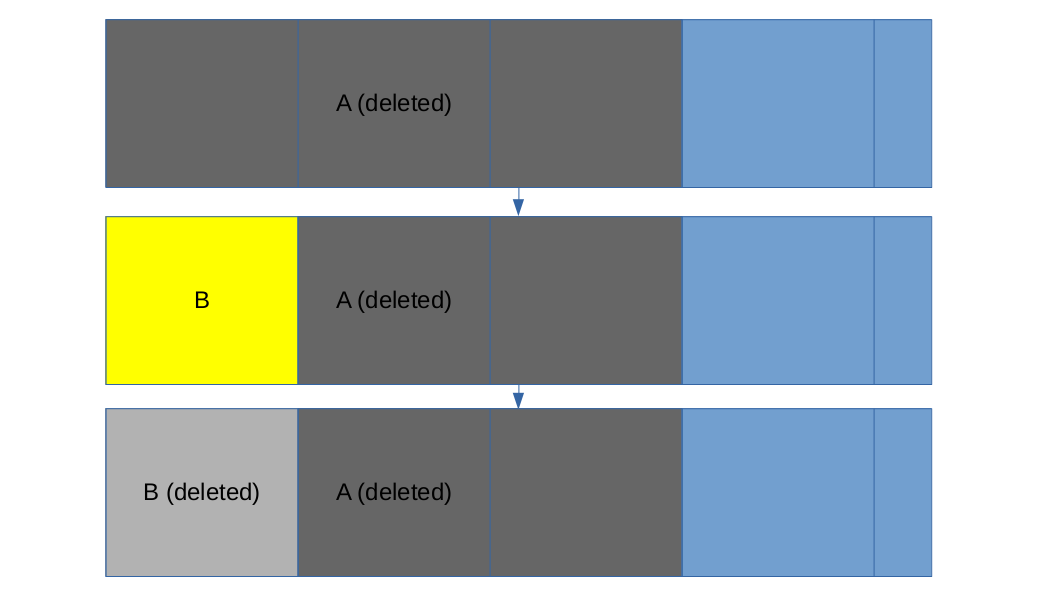
\includegraphics[width=\linewidth]{fig/case5i.png}
%     \caption{Test Case 5i}
%     \label{fig:case_5i}
% \end{figure}

Assuming the file system is NTFS (to avoid the aforementioned ambiguity with core feature 3 and FAT), the residual metadata entry for File A (in this case its Master File Table entry) should list every cluster File A once occupied. 
All of those clusters are unallocated, so to fulfill core feature 3, the tool must recover them. 
However, some of those clusters have been overwritten by File B. Core feature 4 requires that a tool only recover ``data blocks from the Deleted Block Pool,''~\cite{meta:dfr:standards} and defines the Deleted Block Pool as all blocks which ``have not been reallocated or reused.''~\cite{meta:dfr:standards}
Core feature 3 would require tools to recover the clusters reused by File B, while core feature 4 would forbid this. 
It could be argued that the tool should use File B's metadata to recognize that File B overwrote File A, but this is not always realistic. 
While the file system stores information such as creation and modification times, this is not ``essential metadata,'' meaning it is not involved in the operation of the file system, so operating systems may implement it inconsistently, or not at all.~\cite{carrier:filesystems}
Since the time information cannot be counted on to be reliable, there is no way to know for sure which file overwrote which. 
It is also possible for File B's metadata entry to be overwritten at some point before File A's, in which event there is no way for the tool to know File B even existed.

The standards document acknowledges that the ``potential for corruption [is] inherent with data that is no longer maintained by a file system,''~\cite{meta:dfr:standards} and that the recovered object ``may not completely match the original FS-Object.''~\cite{meta:dfr:standards}
We propose the standards themselves should be revised to better account for such situations.
This could mean adding an exception to either the third or fourth core feature, for cases in which data blocks are overwritten and subsequently deallocated.

NIST's James Lyle proposes that rather than deal with the complications involved in accommodating 
many different file systems, standards should be written for ``an ideal file system that leaves in 
residual metadata  all  information  required  to  reconstruct  a  deleted  file''~\cite{lyle2011-ICDF2C}. 
While this can result in tools being held to an impossible standard when using certain file systems, 
Lyle says that is acceptable because the user experience will be the same regardless of whether a feature is impossible or has merely been left out.
If the NIST guidelines were created with such an ideal file system in mind, the current standards may be adequate.
However, that philosophy should be clarified in the guidelines document to avoid confusion.
\end{paraphrase}



% Carving
\subsubsection{False-Positives from File Carving}
% What to do about additional files? It's clear for CR1, but not for the others.
\TODO{still need to write a lead-in to this}

 
Interpreting ``each carved file'' to include even the ones with no relation to the original files results in dramatically low scores for tools like Scalpel (which carved at least 50 additional ``files'' from most of our test images), while favoring tools which are more conservative in their recovery.
However, this would would obscure a relevant trade-off, that a more aggressive tool will have a high false-positive rate, but may recover files that a more conservative tool would miss.
An investigator may have this trade-off in mind when selecting a DFR tool, so the NIST guidelines should not make a tool that lies on one side of that trade-off look objectively worse than others.
As the standards are currently written, a tool that carves only one file from an image, but recovers it correctly, would be considered perfect on four out of five core features.
Meanwhile, a tool that correctly carves all 40 files in an image, but also recovers 100 false-positives, would likely score very poorly for core features 3, 4, and 5.
It would score especially poorly on core feature 5 as false-positives will almost never be a valid file.
Since the NIST guidelines do not directly account for the false-positive rate, it indirectly and disproportionately affects several core features, diluting their usefulness.

To resolve this issue, we propose the following changes to the NIST guidelines:
\begin{arabiclist}
 \item Add a new definition: \emph{Positive Carved File}, a carved file which corresponds to a supported file header signature from a source file that is present in the search arena. \TODO{come up with a better name for this}
 \item In core features 3, 4, and 5, change ``carved file'' to ``positive carved file.''
 \item Add an additional core feature: \emph{The tool shall not return any carved files that do not correspond to a supported file header signature from a source file that is present in the search arena.}
\end{arabiclist}

The intent of these changes is to somewhat atomize the guidelines, so each core feature evaluates a tool on a single capability.
This should make the trade-offs of certain tools more apparent, enabling investigators to make more informed and nuanced tool choices.

\subsection{Related Work}

\section{Conclusion}\label{conclusion}

\section{Acknowledgments}
Acknowledgments to funding bodies etc. may be placed in a separate
section at the end of the text, before the Appendices. This should not
be numbered so use \verb|\section*{Acknowledgements}|.

\section{Appendix}\index{appendix}
Appendices should be used only when absolutely necessary. They
should come before the References.


\bibliographystyle{ws-rv-van}
\bibliography{bibfile}

%\blankpage
%\printindex[aindx]                 % to print author index
%\printindex                        % to print subject index

\end{document} 
